\chapter{Inngangur að skammtafræði}



\begin{tcolorbox}

\iduck{There is nothing new to be discovered in physics now. All that remains is more and more precise measurement.} \\

\vspace{-0.5cm}
\raggedleft{- \textbf{William Thomson (Lord Kelvin), 1900}}
\end{tcolorbox}

\begin{tcolorbox}

\iduck{The task is not so much to see what no one has yet seen; but to think what nobody has yet thought, about that which everybody sees.} \\

\vspace{-0.5cm}
\raggedleft{- \textbf{Erwin Schrödinger, 1925}}
\end{tcolorbox}

\section{Sögulegur inngangur}

Árið 1905 hefur stundum verið kallað \textit{Annus Mirabilis} eða ár undrana því það ár birti Einstein fjórar greinar (tæknilega séð þrjár því fjórða greinin er framhald af þriðju greininni) sem hver er talin marka nýtt upphaf að ólíkum greinum eðlisfræðinnar. Flestir kannast ágætlega við þriðju og fjórðu greinarnar sem fjalla um takmörkuðu afstæðiskenninguna. Færri kannast við aðra greinina um Brown-hreyfingu en það var fyrsta raunverulega röksemdarfærslan fyrir tilvist atóma (þannig var fyrst hægt að mæla stærð þeirra með skipulögðum hætti!). Einstein gaf síðan út almennu afstæðiskenninguna árið 1915 sem útskýrir hvernig að þyngdarkrafturinn virkar (þyngdarlögmál Newtons er nálgun!). Einstein hlaut síðan nóbelsverðlaunin árið 1921, en það er frekar athyglisvert í sögunni, að það var ekki fyrir verk hans á afstæðiskenningunni sem hann er frægastur fyrir í dag heldur var það fyrir fyrstu greinina sem að hann skrifaði árið 1905 um svokallaða ljósröfunartilraun. Í tilkynningu nóbelsnefndarinnar segir nefnilega: \\

\vspace{0.1cm}
 \textit{For his services to Theoretical Physics, and especially for his discovery of the law of the photoelectric effect.}
 \vspace{0.3cm}
 
 En það var fyrsta greinin sem hann birti árið 1905. Hún fjallaði um þessa svokölluðu ljósröfunartilraun. Þessi grein er af mörgum talin marka upphafið að skammtafræði en það er frekar írónískt því Einstein eyddi stórum hluta ævinnar í að reyna að færa rök gegn skammtafræðinni (sbr.~samræður hans við Niels Bohr). Á þessum tímapunkti er kannski allt í lagi að útskýra hvers vegna Einstein var svo mótfallinn skammtafræðinni. Hann á að hafa sagt um skammtafræðina (sem stjórnast af líkum eins og teningakast):
 
\begin{tcolorbox}
\iduck{God does not play dice with the universe.} \\

\vspace{-0.5cm}
\raggedleft{- \textbf{Albert Einstein, 1926}}
\end{tcolorbox}

En helsta ástæðan fyrir því að Einstein var mótfallinn skammtafræðinni var vegna þess að það kemur í ljós að skammtafræðin og almenna afstæðiskenningin eru ekki samrýmanlegar kenningar í þeirri merkingu að það er hægt að sýna fram á að aðeins önnur af þessum tveimur kenningum geti staðist - þær eru semsagt í mótsögn við hvor aðra! Einstein veðjaði auðvitað á að það væri almenna afstæðiskenningin sem að réði ríkjum og að skammtafræðin þyrfti að víkja fyrir betri kenningu. Ein frægasta grein allra tíma er einmitt svokölluð EPR-þversögn (Einstein–Podolsky–Rosen) en í þeirri grein færði Einstein að því er honum virtist óhrekjanleg rök fyrir því að skammtafræðin væri í mótsögn við sjálfa sig. Þetta er reyndar kveikjan afar merkilegum heimspekilgum samræðum og bréfaskrifum sem að danski eðlisfræðingurinn Niels Bohr og Albert Einstein áttu árin 1920-1930 um eðli skammtafræðinnar. Albert Einstein vildi meina að undirliggjandi gæti heimurinn ekki stjórnast af líkum - þetta væri bara galli í kenningunni - okkur vantaði bara nákvæmari lýsingu á heiminum til þess að við gætum útskýrt hvaðan þessar líkur kæmu. Hinsvegar vildu fylgismenn Bohrs meina að það væri aldrei hægt að ákvarða neina nánari lýsingu - efnisheimurinn er handahófskenndur og stjórnast af líkum á dýpsta plani tilverunnar. EPR-þversögnin sem að átti að vera helsti þyrnirinn í augum fylgismanna Niels Bohrs varð þvert á móti helsta vígi þeirra! Árið 1982 birti franski eðlisfræðingurinn Alain Aspect tilraunastaðfestingu á þessari svokölluðu þversögn og sýndi að það væru ekki til neinar huldar breytistærðir eins og Einstein hafði spáð fyrir um!


\section{Glerpíputilraun Faradays}

Til að skilja ljósröfunartilraunina almennilega verðum við að fara aftur til Michael Faradays (já! Það er maðurinn á bak við hið alræmda spanlögmál)\footnote{Reyndar var Michael Faraday afar ofarlega í huga Albert Einstein þegar hann skrifaði greinar sínar árið 1905. Til dæmis hefst greinin hans um afstæðiskenninguna á því að dásama störf Faradays.} En Faraday hafði í kringum árið 1820 verið að skoða eftirfarandi uppstillingu:

\begin{figure}[H]
    \centering
    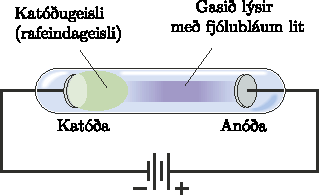
\includegraphics{figures/faraday.pdf}
\end{figure}

Inni í glerpípunni hafði hann komið fyrir gasi (hér neon) og plötum í plötuþétti. Ef að spennumunurinn var nógu mikill á milli platna plötuþéttisins þá kom fram annar grænn geisli inni í glerpípunni sem að hann kallaði katóðugeisla (í dag vitum við að katóðugeislar eru ekkert annað heldur en rafeindageislar). Skoðum þetta aðeins nánar inni í hylkinu. Þegar rafeindirnar rekast á gassameindirnar þá fá sameindirnar orku og örvast upp í hærra orkuástand. En atóm vilja að eðlisfari vera í lægsta orkuástandi sínu, þ.e.~grunnástandinu, svo að atómin reyna að losa sig við orkuna en við það þá geislar atómið frá sér ljóseind með tilheyrandi orku, þ.e.~við höfum að:
\begin{align*}
    E_{\gamma} = \Delta E_{\text{atóm}}
\end{align*}
Það sem meira er: Liturinn á ljósinu sem að gasið gefur frá sér er breytilegur eftir því hvaða efni við erum með inni í glerpípunni. Öfugt þá er hægt að sjá hvaða efni er í hylkinu bara út frá því að litur kemur frá efninu. Sýnilega litrófið samanstendur af ljósi með bylgjulengd:
\begin{align*}
    \lambda_{\text{sýnilegt}} \in \left[ 400;750 \right] \si{nm}.
\end{align*}
En þar sem að $c = \lambda f$ þá samsvarar það eftirfarandi tíðnum:
\begin{align*}
    f_{\text{sýnilegt}} = \frac{c}{\lambda_{\text{sýnilegt}}}  \in \left[ 400; 750 \right] \si{THz}.
\end{align*}
(sem er afar skondin tilviljun!). Hvert efni hefur þá einskonar kennitölu sem kallast litróf frumefnisins og samanstendur af þeim sýnilegu bylgjulengdum sem að efnið getur gefið frá sér. Fyrir vetni höfum við t.d.~að:
\begin{align*}
    \lambda_{\text{H}} \in \left\{ \explain{\SI{410,1}{}}{\text{fjólublár}}; \explain{\SI{434,0}{}}{\text{dökkblár}}; \explain{\SI{486,1}{}}{\text{sægrænn}}; \explain{\SI{656,2}{}}{\text{rauður}} \right\} \si{nm}.
\end{align*}
en fyrir kvikasilfur er t.d.~
\begin{align*}
    \lambda_{\text{Hg}} \in \left\{ \explain{\SI{404,7}{}}{\text{fjólublár}}; \explain{\SI{407,8}{}}{\text{ljós fjólublár}}; \explain{\SI{435,8}{}}{\text{dökkblár}}; \explain{\SI{546,1}{}}{\text{grænn}}; \explain{\SI{577,0}{}}{\text{gulur}}; \explain{\SI{579.1}{}}{\text{appelsínugulur}}\right\} \si{nm}.
\end{align*}
Á þessum tímapunkti förum við að sjá ummerki um skömmtun! Litrófslínurnar geta bara komið í ákveðnum gildum en ekki með hvaða gildi sem er! Þetta er fyrsta vísbendingin um skömmtun á orku atómanna! Þetta minnir á grunnhleðsluna, $e$, en allar hleðslur, $Q$, þurfa að vera heiltölumargfeldi af $e$, þ.e.~til er $N \in \Z$ þannig að $Q = Ne$.


\section{Ljósröfunartilraunin og útskýring Einsteins}

Árið 1886 prufaði Heinrich Hertz að breyta glerpíputilrauninni örlítið þannig að:

\begin{figure}[H]
    \centering
    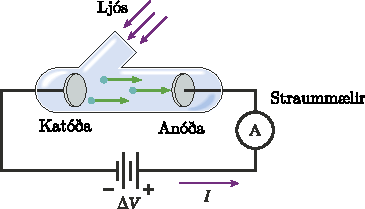
\includegraphics{figures/photoelectric1.pdf}
\end{figure}

Það sem að hann komst að var að ljóseindirnar gátu búið til straum í rásinni en það ætti ekki að vera neinn straumur í rásinni þegar að þéttirinn er fullhlaðinn! Hvernig væri hugsanlega hægt að útskýra það? Það sem meira var, það var bara fyrir ákveðnar bylgjulengdir á ljósi sem að þetta var hægt! Ef að bylgjulengdin var of há þá var ekki hægt að fá straum í rásina sama hversu mikill ljósstyrkurinn var en um leið og bylgjulengdin varð nógu lág (og þar með hækkaði orka ljóseindanna í ljósinu) þá var hægt að fá straum í rásina. Hertz skráði niður athuganir sýnar:

\begin{enumerate}[label =  (\arabic*)]
    \item Ljósröfunarstraumurinn í rásinni er í beinu hlutfalli við ljósstyrkinn.
    
    \item Straumurinn í rásinni byrjar um leið ($< \SI{1}{ns}$) og kveikt er á ljósinu.
    
    \item Ljósröfunarstraumurinn kemur einungis fram ef tíðni ljóssins er $f > f_0$ eða $\lambda < \lambda_0$ þar sem $f_0$ kallast \textbf{þröskuldstíðni málmsins} og er háð efninu sem að plötuþéttirinn samanstendur af.
    
    \item Ef að rafhlöðunni er snúið við og ljósinu beint að jákvæðu plötu plötuþéttisins þá hættir straumurinn í rásinni þegar að spennumunurinn í rásinni verður $V_{\text{þ}}$, þar sem að $V_{\text{þ}}$ kallast \textbf{þröskuldsspenan}. Gildið á $V_{\text{þ}}$ er breytilegt eftir efnum og óháð ljósstyrknum. Með öðrum orðum, sama hversu sterkt ljósið er þá endar spennumunurinn í rásinni alltaf í $V_{\text{þ}}$.
\end{enumerate}

Einstein hlaut nóbelsverðlaunin árið 1921 fyrir að útskýra þessa ljósröfunartilraun. Einstein lagði til að orka ljóss væri skömmtuð. Hann kallaði slíkan orskuskammt ljóseindir. Hann staðhæfði að:
\begin{align*}
    E_\gamma = hf
\end{align*}
þar sem að $h = \SI{6.626e-34}{Js}$ er fasti Plancks.\footnote{Fastinn, $h$, heitir eftir þýska eðlisfræðingnum Max Planck sem notaði hann fyrst árið 1900 til að útskýra svarthlutsgeislun (sem útskýrir djúpstæð tengsl milli litrófslína og hitastigs). En Planck notaði tilgátuna hans Einsteins án þess að átta sig á því!} Þá gat Einstein útskýrt ljósröfunina með eftirfarandi hætti:

\begin{figure}[H]
    \centering
    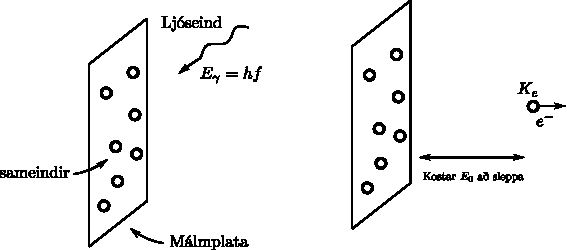
\includegraphics{figures/einstein-uts.pdf}
\end{figure}

Til þess að osa rafeind frá yfirborðinu á málminum þá þarf örvaða rafeindin (sem gleypir ljóseindina) að fá nógu mikla orku til þess að yfirvinna alla rafsegulkraftana sem að halda henni í málmplötunni. Því er til minnsta orka; svokallað vinnufall mámlsins (sem er breytilegt fyrir mismunandi málma), $E_0$, þannig að:
\begin{align*}
    E_\gamma = E_0 + K_e \hspace{0.5cm} \text{þ.e.} \hspace{0.5cm} K_e = E_\gamma - E_0 = hf - hf_0 = h(f-f_0).
\end{align*}
þar sem að $K_e$ táknar hreyfiorku rafeindarinnar sem að losnar. En þá nær rafeindin bara að lenda á neikvæðu plötu plötuéttisins ef að hún hefur nægilega orku til að yfirvinna rafsviðið (sem er að reyna að stöðva hana) sem gefur því að þröskuldsspennan verður
\begin{align*}
    eV_{\text{þ}} = K_e = hf - E_0.
\end{align*}


\section{Efnisbylgjur de Broglie}

Samkvæmt afstæðiskenningu Einsteins er orku-skriðþunga jafnan:
\begin{align*}
    E^2 = E_0^2 + (pc)^2
\end{align*}
þar sem að $E$ táknar heildarorku eindarinnar, $E_0$ táknar kyrrstöðuorku eindarinnar og $p$ táknar skriðþunga eindarinnar. Ljóseindir eru massalausar og fyrir þær gildir að $E_0 = 0$ en þar með höfum við að:
\begin{align*}
    E_\gamma = p_\gamma c \implies p_\gamma = \frac{E_\gamma}{c} = \frac{hf}{c} = \frac{\frac{hc}{\lambda}}{c} = \frac{h}{\lambda}.
\end{align*}
Með öðrum orðum þá höfum við almennt að skriðþungi ljóseindar er gefinn með:
\begin{align*}
    p_\gamma = \frac{h}{\lambda}.
\end{align*}
En árið 1924 í doktorsritgerðinni sinni þá staðhæfði Louis de Broglie (borið fram du broj) að sama jafn gildir líka fyrir efnisagnir. Þ.e. til er svokölluð de Broglie bylgjulengd fyrir allar efnisagnir sem er gefin með:
\begin{tcolorbox}
\begin{align*}
    \lambda = \frac{h}{p}.
\end{align*}
\end{tcolorbox}
Þar sem að $p = mv$ eða $p = \gamma mv$ (eftir því hvort á betur við) er skriðþungi efniseindarinnar. \\

Hann notaði þetta til þess að útskýra mörg skammtafræðileg fyrirbæri (hann hlaut nóbelsverðlaunin árið 1929 fyrir störf sín með efnisbylgjur). En sér í lagi notaði hann þetta til þess að útskýra kjarnann og atómið. Hann ímyndaði sér nefnilega að kjarninn væri eins og kassi og að kjarneindirnar gætu einungis hegðað sér eins og staðbylgjur á streng inni í kassanum (með lokuðu jaðarskilyrði því kassinn er lokaður).

\begin{figure}[H]
    \centering
    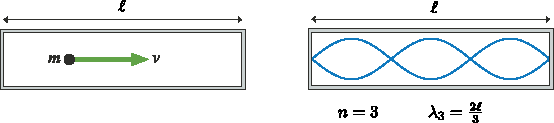
\includegraphics{figures/stadbylgja.pdf}
\end{figure}

Hryefiorka agnanna í kassanum er
\begin{align*}
    K = \frac{1}{2}mv^2 = \frac{p^2}{2m}.
\end{align*}
Þar að auki sem að samkvæmt bylgjuagnaforsendu de Broglie er $\lambda = \frac{p}{h}$ svo:
\begin{align*}
    K = \frac{\left( \frac{h}{\lambda} \right)^2}{2m} = \frac{h^2}{2m} \frac{1}{\lambda^2}
\end{align*}
En staðbylgjur uppfylla þá að $\lambda = \frac{2\ell}{n}$ þar sem $n \in \Z_+$ svo 
\begin{align*}
    E_n = K_n = \frac{h^2 n^2}{8m\ell^2}
\end{align*}
er heildarorka agnanna í kassanum. Við sjáum þá sér í lagi að orkan er skömmtuð. 

\section{Klassískur líftími atómsins (*)}

Árið 1913 settu Daninn Niels Bohr og Ernest Rutherford fram nýtt atómlíkan.
Hugmyndir þeirra byggðu ofan á plánetulíkani Rutherfords af atóminu frá árinu 1911 (í rauninni er lítill munur á líkönunum).
Einstein hafði árið 1905 lagt til að ljós samanstæði af litlum ögnum sem hann kallaði ljóseindir (\emph{light quanta}). Bein þýðing væri hugsanlega ljósskammtar.
Samkvæmt Einstein var orka ljóseindar skömmtuð og gefin með $E_\gamma = hf$ og skriðþungi ljóseindar ákvarðast af $E^2 = \explain{E_0^2}{=0} + (pc)^2$ þ.a. $E_\gamma = p_\gamma c$ fyrir ljós (hér höfum við notað að ljóseindir eru massalausar).
Helsti gallinn við atómlíkan Rutherfords var að það var bersýnileg mótsögn í því. Samkvæmt klassískri eðlisfræði mun ögn með hleðslu $q$ sem verður fyrir hröðun geisla frá sér orku (tapar orku) með afli:

\begin{align*}
    P_L = \frac{q^2a^2}{6\pi \epsilon_0 c^3}, \hspace*{3cm} \text{(Larmor jafnan)}
\end{align*}
En það þýðir að rafeindin sem er á hringhreyfingu um róteindina ætti að tapa orku og spírala inn að kjarnanum:
\begin{figure}[H]
    \centering
    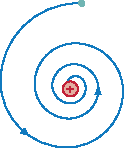
\includegraphics{figures/spirala.pdf}
\end{figure}
Þannig getum við metið líftíma atómsins. Það er að segja við getum metið hversu langur tími líður þar til að rafeindin hefur spíralað inn í kjarnann. Við athugum þá að kraftajafnan gefur:
\begin{align*}
    m_e \frac{v^2}{r} = \frac{ke^2}{r^2} \implies \frac{v^2}{r} = \frac{ke^2}{m_er^2}
\end{align*}
þ.a.
\begin{align*}
    P = - \frac{dE}{dt} = \frac{e^2 \left( \right)^2}{4\pi \epsilon_0 c^3} = \frac{k^2 e^6}{4\pi \epsilon_0 m_e^2 c^3} \frac{1}{r^4}
\end{align*}
En við athugum líka að:
\begin{align*}
    E = \frac{1}{2}mv^2 - \frac{ke^2}{r} = -\frac{ke^2}{2r}
\end{align*}
Þannig að við höfum samkvæmt keðjureglunni að:
\begin{align*}
    \frac{dE}{dt} = \frac{dE}{dr} \cdot \frac{dr}{dt} = \frac{d}{dr}\left( -\frac{ke^2}{2r} \right) \cdot \frac{dr}{dt} = \frac{ke^2}{2r^2} \frac{dr}{dt}.
\end{align*}
En þar með höfum við sýnt að:
\begin{align*}
    P_L = -\frac{dE}{dt} = -\frac{ke^2}{2r^2}\cdot \frac{dr}{dt} = \frac{k^2e^6}{4\pi \epsilon_0 m_e^2 c^3} \cdot \frac{1}{r^4}
\end{align*}
þ.a.
\begin{align*}
    \frac{dr}{dt} = -\frac{ke^4}{2\pi \epsilon_0 m_e^2 c^3} \cdot \frac{1}{r^2}
\end{align*}
Sem við leysum með tegrun:
\begin{align*}
    -\int_{a}^{b} r^2 dr = \int_{0}^{\tau} \frac{ke^4}{2\pi \epsilon_0 m_e^2 c^3}dt \implies \left[ \frac{1}{3}r^3 \right]_{a}^{b} = \left[ \frac{ke^4}{2\pi \epsilon_0 m_e^2 c^3} t  \right]_{0}^{\tau} \implies \frac{a^3-b^3}{3} = \frac{ke^4}{2\pi \epsilon_0 m_e^2 c^3} \tau
\end{align*}
Svo líftimi atómsins er:
\begin{align*}
    \tau = \frac{2}{3} \cdot \frac{\pi \epsilon_0 m_e^2 c^3}{ke^4} \left( a^3 - b^3 \right) = \SI{10}{ps}
\end{align*}
Þar sem við höfum notað $a = \SI{0.529}{\AA}$ og $b = \SI{1.2}{fm}$. Þetta er bersýnileg mótsögn því annars hefðu öll atómin sem að við samanstöndum úr hrörnað nú þegar og við værum því ekki til!

\section{Bohr-líkanið}

En danski eðlisfræðingurinn (og nóbelsverðlaunahafi 1922) reyndi að lagfæra þetta gallaða atómlíkan árið 1913 með eftirfarandi þremur forsendum:

\begin{tcolorbox}
\textbf{Frumsendur að atómlíkani Bohrs}
\begin{enumerate}[label = \textbf{(\roman*)}]
    \item Rafeindin er á stöðugri hringhreyfingu umhveris kjarnan án þess þó að geisla frá sér orku. Þessar brautir eru skammtaðar í þeirri merkingu að rafeindin getur einungis verið í ákveðinni fjarlægð frá róteindinni (en ekki hvaða fjarlægð sem er).
    
    \item Þessar stöðugu brautir eru þær brautir þar sem að hverfiþungi rafeindarinnar á sporbraut hennar um kjarnan er skammtaður þannig að:
    \begin{align*}
        L = n \hbar 
    \end{align*}
    Þar sem $\hbar = \frac{h}{2\pi} = \SI{1.05e-34}{Js}$ er fasti sem nefnist smækkaður Plancks-fasti (eða há-slá).
    
    \item Rafeindir geta einungis stokkið á milli leyfilegra brautargeisla með því annað hvort að taka við eða geisla frá sér rafsegulgeislun (ljóseind) með orku $\Delta E_{\text{atóm}} = E_\gamma = hf$.
\end{enumerate}
\end{tcolorbox}

Þessi skammtatilgáta hófst með Planck og Einstein árið 1905. En Einstein hafði haft þá tilgátu að líta mætti á sem svo að ljós samanstæði af svokölluðum ljóseindum þar sem að hver ljóseind hefði orku $E = hf$ þar sem $h = $ var Plancks-fastinn og $f$ var tíðni ljóssins.

Samkvæmt atómlíkani Bohrs þá gildir því að:
\begin{align*}
    m a = m \frac{v^2}{r} = \frac{ke^2}{r^2} \implies v = \sqrt{\frac{ke^2}{m r}}
\end{align*}
En þar með höfum við að þar sem að hverfiþungi agnarinnar er heiltölumargfeldi af smækkaða Plancks-fastanum að:
\begin{align*}
    mvr = n\hbar \implies m \sqrt{\frac{ke^2}{mr}} r = n \hbar \implies mke^2 r = n^2 \hbar^2 \implies r_n = \frac{\hbar^2 n^2}{mke^2} = a_B n^2.
\end{align*}
Þar sem $a_0 = r_1 = \SI{0.529}{\AA}$ er svokallaður Bohr-geisli og táknar minnstu leyfilegu brautarvegalengdina sem að rafeindin getur haft. En þá sjáum við að brautarhraði rafeindarinnar á $n$-tu braut er gefinn með:
\begin{align*}
    v_n = \sqrt{\frac{ke^2}{mr_n}} = \sqrt{\frac{ke^2}{ma_B}} \cdot \frac{1}{n} = \frac{v_1}{n} 
\end{align*}
þar sem $v_1 = \SI{2.19e6}{m/s}$ er brautarhraði rafeindarinnar á innsta hveli. Heildarorka rafeindarinnar á $n$-tu braut er þá gefin með:
\begin{align*}
    E_n = \frac{1}{2}m_ev_n^2  - \frac{ke^2}{r_n} = \frac{1}{2} m_e \frac{ke^2}{m_e r_n} - \frac{ke^2}{r} = -\frac{1}{2} \frac{ke^2}{r_n} = -\frac{E_1}{n^2}
\end{align*}
Þar sem $E_1 = \SI{13.6}{eV}$ er heildarorka rafeindarinnar á innsta hveli (takið eftir því að heildarorka rafeindarinnar er alltaf neikvæð og því ytra sem að rafeindin fer því nær kemst heildarorkan núlli). En þar með ályktum við að orkan sem að rafeindin geislar frá sér við það að fara á milli orkuhvela er gefin með:
\begin{align*}
    \frac{hc}{\lambda} = hf = \Delta E = E_m - E_n = -\frac{E_1}{m^2} + \frac{E_1}{n^2} = -E_1 \left( \frac{1}{m^2} - \frac{1}{n^2} \right)
\end{align*}
En þar með ályktum við að gleypnilínur vetnisatómsins verða greinilegar við eftirfarandi bylgjulengdir:
\begin{align*}
    \lambda = \frac{-\frac{hc}{E_1}}{\left( \frac{1}{m^2} - \frac{1}{n^2} \right)} = \frac{\lambda_0}{\left( \frac{1}{m^2} - \frac{1}{n^2} \right)}
\end{align*}
Þannig tókst Bohr að spá fyrir gleipnilínurófi vetnisatómsins. En þegar að Bohr reyndi að framkvæma sömu reikninga fyrir helín atómið þá voru niðurstöðurnar hans algjörlega í mótsögn við mælingar. Hann hafði því gert eitthvað rétt en samt svo vitlaust!



\section{Óendanlegur mættisbrunnur}

Lítum á eind með massa $m$ og hraða $v$ sem að ferðast inni í kassa með lengd $\ell$. Samkvæmt de Broglie hefur eindin einhverja bylgjulengd:
\begin{align*}
    \lambda = \frac{h}{p} = \frac{h}{mv}.
\end{align*}
En við höfum áður lært að staðbylgjur með lokuð jaðarskilyrði uppfylla:
\begin{align*}
    \lambda_n = \frac{2\ell}{n}
\end{align*}
Með því að setja þessar tvær hugmyndir saman þá ályktum við að:
\begin{align*}
    \frac{2\ell}{n} = \frac{h}{mv_n} \implies v_n = \frac{hn}{2m\ell}
\end{align*}
Heildarorka eindarinnar inni í kassanum er einungis vegna hreyfiorku hennar svo að við höfum því að:
\begin{align*}
    E_n = \frac{1}{2}mv_n^2 = \frac{1}{2}m \left( \frac{hn}{2m\ell} \right)^2 = \frac{h^2n^2}{8m\ell^2}.
\end{align*}

Tilheyrandi bylgjuföll verða þá:
\begin{align*}
    \psi_n(x) = A\sin(k_nx) = A\sin\left(\frac{2\pi x}{\lambda_n}\right) = A\sin\left( \frac{\pi n x}{\ell} \right)
\end{align*}
Við tengjum við bylgjufallið svokallaðan líkindaþéttleika:
\begin{align*}
    \rho_n(x) = \abs{\psi_n(x)}^2 = A^2 \sin^2\left( \frac{\pi n x}{\ell} \right)
\end{align*}
Líkindaþéttleikinn lýsir líkunum á því að finna ögnina inni á einhverju bili með eftirfarandi hætti:
\begin{align*}
    \mathds{P}_{[a,b]} = \int_{a}^{b} \rho(x)dx  
\end{align*}
Heildarlíkurnar á því að finna ögnina inni í kassanum verða því að vera $1$ þannig að við höfum að:
\begin{align*}
    1 = \mathds{P}_{[0,\ell]} = \int_{0}^{\ell} A^2 \sin^2\left(\frac{n\pi x}{\ell}\right)dx = A^2 \int_{0}^{\ell} \frac{1-\cos\left(\frac{2n\pi x}{\ell}\right)}{2} dx = \frac{A^2}{2}\left[ x - \frac{\ell}{2 \pi n} \sin\left(\frac{2 n \pi x}{\ell}\right) \right]_{0}^{\ell} = \frac{A^2 \ell}{2}
\end{align*}
Svo við ályktum að:
\begin{align*}
    A = \sqrt{\frac{2}{\ell}}.
\end{align*}
Við höfum þar með að bylgjuföllin verða:
\begin{align*}
    \psi_n(x) = \sqrt{\frac{2}{\ell}} \sin\left( \frac{2\pi n x}{\ell} \right), \hspace{1cm} \text{og líkindaþéttleikinn verður} \hspace{1cm} \rho_n(x) = \frac{2}{\ell}\sin^2\left( \frac{n\pi x}{\ell} \right).
\end{align*}
Við getum þá svarað spurningum eins og:

\begin{itemize}
    \item Hverjar eru líkurnar á því að finna ögn í skammtaástandi $n$ milli $\frac{\ell}{4}$ og $\frac{\ell}{2}$?
\end{itemize}

\textbf{Lausn:} Höfum þá:
\begin{align*}
    \mathds{P}_{[\frac{\ell}{4},\frac{\ell}{2}]} &= \int_{\ell/4}^{\ell/2} \rho_n(x) = \frac{2}{\ell} \int_{\ell/4}^{\ell/2} \sin^2\left(\frac{n\pi x}{\ell} \right)dx = \frac{1}{2\ell} \int_{\ell/4}^{\ell/2} \left( 1 - \cos\left( \frac{2 \pi n x}{\ell} \right) \right)dx \\
    &= \frac{1}{2\ell} \left[ x - \frac{\ell}{2\pi n} \sin\left(\frac{2\pi n x}{\ell}\right) \right]_{\ell/4}^{\ell/2} \\
    &= \frac{1}{2\ell} \left( \frac{\ell}{2} - \frac{\ell}{4} - \frac{\ell}{2\pi n} \sin(n\pi ) + \frac{\ell}{2\pi n} \sin\left(n\frac{\pi}{2}\right) \right) \\
    &= \frac{1}{2}\left( \frac{1}{4} + \frac{1}{2\pi n}(-1)^{n+1} \right).
\end{align*}

\begin{comment}
\section{Óvissulögmál Heisenbergs}

Áður en að við byrjum að fjalla um óvissulögmálið þá skulum við staldra aðeins við og skoða þessi góðu jörm:

\begin{figure}[H]
    \centering
    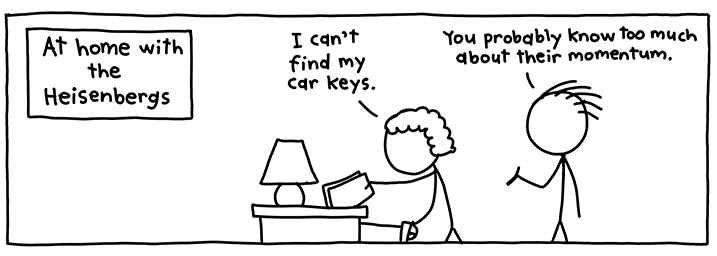
\includegraphics[width = 0.7\textwidth]{figures/guest.png}
\end{figure}

\begin{figure}[H]
    \centering
    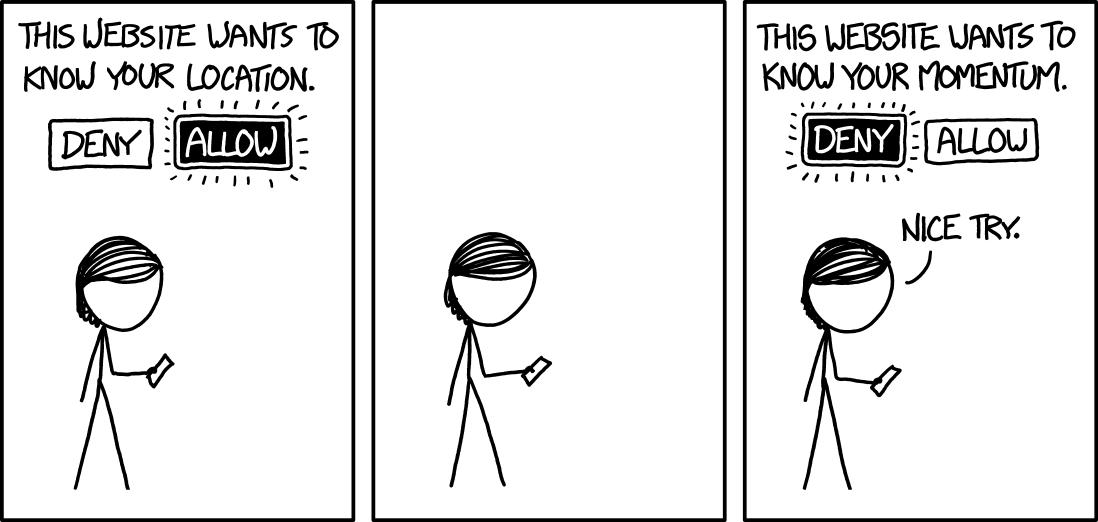
\includegraphics[width = 0.7\textwidth]{figures/loc.png}
\end{figure}


\section{Schrödinger-jafnan}

Við byrjum á því að skoða hefðbundnu jöfnuna fyrir orku, þ.e.
\begin{align*}
    E = \frac{1}{2}mv^2 + U = \frac{p^2}{2m} + U(x),
\end{align*}
þar sem $p$ táknar skriðþunga agnar með massann $m$ og $U$ er stöðuorkan sem ögnin finnur fyrir. Hér höfum við takamarkað okkur við ögn sem hreyfist í einni vídd og munum glíma við fleiri víddir síðar. Við uppfærum $E$ og $p$ yfir í skammtavirkja $\hat{E}$ og $\hat{p}$ sem eru þannig að
\begin{align*}
    \hat{E} = i\hbar \pdv{}{t}, \hspace{0.8cm} \hat{p} = -i\hbar\pdv{}{x}.
\end{align*}
Við stingum þessu inn í staðinn fyrir stærðirnar í upphaflegu orkujöfnunni og látum báðar hliðar verka á bylgjufallið $\Psi = \Psi(x,t)$. Þá höfum við:
\begin{align*}
    i\hbar \pdv{\Psi}{t} = \left(\frac{1}{2m}\left( -i\hbar \pdv{}{x} \right)^2 + U(x) \right)\Psi
\end{align*}
Það er að segja
\begin{align*}
  i\hbar \pdv{\Psi}{t} = -\frac{\hbar^2}{2m} \pdv[2]{\Psi}{x} + U(x) \Psi.
\end{align*}
Jafnan hér að ofan kallast tímaháða Schrödinger-jafnan. En fólki finnst almennt flókið að vinna bæði með tímaafleiður og rúmafleiður í einu svo að það er til smá trikk til þess að losna við það! Við notum aðskilnað breytistærða en það þýðir að við skrifum:
\begin{align*}
    \Psi(x,t) = \psi(x)\varphi(t)
\end{align*}
og stingum því inn í Schrödinger-jöfnuna:
\begin{align*}
    i \hbar \pdv{}{t} \Big(\psi(x)\varphi(t)\Big) = - \frac{\hbar^2}{2m} \pdv[2]{}{x} \Big(\psi(x)\varphi(t)\Big) + U(x)\psi(x)\varphi(t)
\end{align*}
Eftir að við diffrum höfum við að:
\begin{align*}
    i\hbar \psi(x) \pdv{\varphi}{t} = -\frac{\hbar^2}{2m} \varphi(t) \pdv[2]{\psi}{x} + U(x)\psi(x)\varphi(t)
\end{align*}
Við deilum síðan í gegn með $\psi(x) \varphi(t)$ og höfum:
\begin{align*}
   i \hbar \frac{\pdv{\varphi}{t}}{ \varphi(t)} = -\frac{\hbar^2}{2m} \frac{\pdv[2]{\psi}{x}}{\psi(x)} + U(x)
\end{align*}
En þá sjáum við að vinstri hliðin er einungis háð $t$ og hægri hliðin er einungis háð $x$ en eina leiðin til þess að það gangi upp er ef að báðar hliðar eru fastar! Með öðrum orðum þá er til fasti $E$ (forsjált) þannig að:
\begin{align*}
    i \hbar \frac{\pdv{\varphi}{t}}{ \varphi(t)} = E = -\frac{\hbar^2}{2m} \frac{\pdv[2]{\psi}{x}}{\psi(x)} + U(x)
\end{align*}
Ef við umritum þetta þá höfum við semsagt tvær diffurjöfnur:
\begin{align*}
    i\hbar \pdv{\varphi}{t} = E\varphi(t), \hspace{1cm} \text{og} \hspace{1cm} -\frac{\hbar^2}{2m} \pdv[2]{\psi}{x} + U(x)\psi(x) = E\psi(x).
\end{align*}
Fyrri diffurjafnan er fyrsta stigs diffurjafna með fastastuðlum og því auðleyst:
\begin{align*}
    \varphi(t) = \varphi_0 e^{-iEt/\hbar}
\end{align*}
þar sem $\varphi_0$ er fasti sem ákvarðast af upphafsskilyrðinu. Seinni diffurjafnan kallast tímaóháða Schrödingerjafnan (af því að það eru engar tímaafleiður í henni) og það er almennt vandasamt að leysa hana nema í örfáum sértilvikum þar sem að stöðuorkan, $U(x)$, er afar einföld.

\section{Óendanlegur mættisbrunnur (aftur)}

Við skulum núna sýna hvernig að óendanlegi mættisbrunnurinn er leystur með almennu Schrödingerjöfnunni. Látum mættisbrunninn vera í $[0,\ell]$. Við getum ímyndað okkur að þetta sé eins og kassi með þykka veggi sem ögnin getur ekki sloppið út um (sjáum síðar undir hvaða kringumstæðum hún getur sloppið). Stöðuorkan er þá gefin með gaffalforskrift:
\vspace{-0.3cm}
\begin{align*}
    U(x) = \begin{cases} 
    0 & \text{ef } x \in [0,\ell] \\
    +\infty & \text{ef } x \not\in [0,\ell] \\
    \end{cases}
\end{align*}
Þegar að við stingum þessu inn í tímaóháðu Schrödinger-jöfnuna þá fáum við:
\begin{align*}
    -\frac{\hbar^2}{2m} \pdv[2]{\psi}{x} = E\psi(x) \implies \pdv[2]{\psi}{x} = -\frac{2mE}{\hbar^2}\psi(x)
\end{align*}
Sem er einföld sveifluhreyfing svo við látum $k = \sqrt{\frac{2mE}{\hbar^2}}$. Lausnin er þá gefin með:
\begin{align*}
    \psi(x) = A\cos(kx) + B\sin(kx)
\end{align*}
Við höfum síðan jaðarskilyrði í $\psi(0)$ og $\psi(\ell)$. Við vitum nefnielga að ögnin verður að samsvara staðbylgju sem er bundin í báða endana svo þetta eru lokuð jaðarskilyrði með $\psi(0) = \psi(\ell) = 0$ (Önnur meira fancy leið til þess að sjá þetta er að skoða lausn bylgjujöfnunnar fyrir utan brunninn - þar verður bylgjufallið að vera núll alls staðar og þar sem að bylgjufallið verður að vera samfellt þá gefur markgildið frá vinstri í $0$ og markgildið frá hægri í $\ell$ að bylgjufallið verði að vera núll í þeim punktum). En þar með höfum við af jarðarskilyrðunum að:
\vspace{-0.3cm}
\begin{align*}
    \psi(0) = 0 \implies A = 0.
\end{align*}
Þannig að $\psi(x) = B\sin(kx)$. En síðan höfum við að:
\begin{align*}
    \psi(\ell) = 0 \implies B\sin(k\ell) = 0
\end{align*}
Við gætum auðvitað sett $B = 0$ en það samsvarar leiðinlegu núlllausninni (það eru bara stærðfræðingar sem hafa einhvern áhuga á svona leiðinlegum lausnum). Eina leiðin til þess að fá áhugaverðar lausnir er ef að:
\begin{align*}
    k\ell = n\pi, \hspace{1cm} n \in \Z.
\end{align*}
Við erum semsagt búin að skammta leyfilegu gildin á $k_n$, þ.e.a.s.~við höfum að:
\begin{align*}
    k_n = \frac{n\pi}{\ell}, \hspace{1cm} n \in \Z.
\end{align*}
En þetta er áhugavert því við höfðum þegar sýnt að:
\begin{align*}
    k = \sqrt{\frac{2mE}{\hbar^2}} \implies E_n = \frac{\hbar^2 k^2}{2m} = \frac{\hbar^2 \pi^2 n^2}{2m\ell^2}.
\end{align*}
Með því að nota að $\hbar = \frac{h}{2\pi}$ þá getum við umritað þetta yfir á sama form og við höfðum áður:
\begin{align*}
    E_n = \frac{h^2 n^2}{8m\ell^2}.
\end{align*}
Hér sjáum við þá líka að bylgjuföllin verða:
\begin{align*}
    \psi_n(x) = B\sin(k_nx) = B\sin(\frac{n\pi x}{\ell})
\end{align*}
Stærðin $\rho(x) = \abs{\psi(x)}^2$ er svokallaður líkindaþéttleiki og við höfum þá þar sem að heildarlíkurnar á því að finna ögnina í brunninum eru $1$, að:
    \begin{align*}
    1 = \mathds{P}_{[0,\ell]} = \int_{0}^{\ell} B^2 \sin^2\left(\frac{n\pi x}{\ell}\right)dx = B^2 \int_{0}^{\ell} \frac{1-\cos\left(\frac{2n\pi x}{\ell}\right)}{2} dx = \frac{B^2}{2}\left[ x - \frac{\ell}{2 \pi n} \sin\left(\frac{2 n \pi x}{\ell}\right) \right]_{0}^{\ell} = \frac{B^2 \ell}{2}
\end{align*}
Sem gefur því að stöðlunarfastinn er $B = \sqrt{\frac{2}{\ell}}$ þannig að:
\begin{align*}
    \psi_n(x) = \sqrt{\frac{2}{\ell}} \sin(\frac{n \pi x}{\ell})
\end{align*}


\section{Óvissulögmál Heisenbergs}

Þetta gefur okkur síðan skemmtilega leið til þess að meta stærð atómkjarnans. Hugsum um vetnisatómið þar sem ein rafeind er bundin við eina róteind. Við hugsum okkur að staðsetning rafeindarinnar sé eitthvað líkindaský í kringum kjarnann en það þýðir að meðaltali þá er rafeindin stödd í fjarlægð $r = 0$ frá kjarnanum (þetta gildir líka fyrir rafeind á hringhreyfingu umhverfis kjarnann). Það sama má segja um skriðþunga rafeindarinnar hann er að meðaltali $p = 0$. En samkvæmt óvissulögmáli Heisenbergs þá er alltaf einhver óvissa á staðsetningu agnarinnar svo að meðaltali þá ættum við að segja að fjarlægðin sé $r = 0 \pm \Delta r$ og skriðþunginn sé $p = 0 \pm \Delta p$. En þá höfum við samkvæmt óvissulögmálinu að:
\begin{align*}
    \Delta r \Delta p \geq \frac{\hbar}{2} \implies p = \Delta p = \frac{\hbar}{2 \Delta r} = \frac{\hbar}{2 r}
\end{align*}
En þar með höfum við að heildarorka atómsins er gefin með:
\begin{align*}
    E(r) = \frac{1}{2}mv^2 - \frac{ke^2}{r} = \frac{p^2}{2m} - \frac{ke^2}{r} = \frac{\hbar^2}{4mr^3} - \frac{ke^2}{r}.
\end{align*}
En við vitum að atómið vill vera í orkulægsta ástandinu sínu svo við höfum að:
\begin{align*}
    \frac{dE}{dr} = -\frac{\hbar^2}{4mr^3} + \frac{ke^2}{r^2} \stackrel{!}{=} 0 \implies r = \frac{\hbar^2}{4mke^2} = \SI{0.132}{\AA}.
\end{align*}
\end{comment}

\newpage

\section{Dæmi}

\subsection*{Dæmatími 43: Inngangur að skammtafræði: Ljóseindir og ljósröfun}

\begin{tcolorbox}
Árið 1905 setti Einstein fram tilgátu um eðli ljóssins sem markaði tímamót í sögu eðlisfræðinnar. Hann staðhæfði að ljós samanstæði af litlum orkuskömmtum sem hann kallaði ljóseindir með orku:
\begin{align*}
    E_\gamma = hf = \frac{hc}{\lambda}
\end{align*}
Hann notaði þetta til þess að útskýra eina helstu ráðgátu þess tíma, nefnilega ljósröfun rafeinda úr málmi, en rafeindirnar losna með hreyfiorku:
\begin{align*}
    K_e = E_{\gamma} - E_0 = hf - E_0.
\end{align*}
Þar sem $E_0$ er lágmarksorkan sem þarf til þess að losa rafeindina úr málminum (stundum kallað vinnufall málmsins). Þetta er stundum sett fram í tengslum við svokallaða stöðvunarspennu eða þröskuldsspennu, $V_{\text{þ}}$, en það er spennan sem þarf til þess að stöðva aftur rafeindina sem losnar þannig $K_e = eV_{\text{þ}}$.
\end{tcolorbox}

\begin{enumerate}[label = \textbf{(\alph*)}]

\item[\textbf{(38.7)}] 
\begin{enumerate}[label = \textbf{(\alph*)}]
\item Hver er bylgjulengd ljóseindar sem hefur orku \SI{1.5}{eV}? Er þetta í sýnilega litrófinu?
\item Ljóseind hefur bylgjulengd $\SI{550}{nm}$. Hver er orka ljóseindarinnar?
\item Útvarpsstöðin FM957 sendir út rafsegulbylgjur með tíðni $\SI{95.7}{MHz}$. Hver er orka ljóseindanna?
\item Gammageislar hafa bylgjulengd sem er minni en $\SI{100}{pm}$. Hver er minnsta orka ljóseindanna?
\end{enumerate}

\item[\textbf{(38.12)}] Færustu eðlisfræðingar sögunnar hafa fórnað heilsunni til þess að uppgötva leyndardóma alheimsins. Frægasta dæmið er að finna hjá Marie Curie sem handlék geislavirk efni á hverjum degi í rannsóknum sínum. Annað gott dæmi er að finna hjá Isaac Newton sem missti sjónina í heila viku eftir að hafa verið að gera rannsóknir á sólarljósi. Matti er að reyna að feta í fótspor þessara goðsagna. Hann tekur ólöglegan \SI{500}{mW} rauðan leisi með bylgjulengd $\SI{650}{nm}$ og beinir honum inn í augun á sér í von um að verða frækinn eðlisfræðingur. Hversu margar ljóseindir sendir leisirinn frá sér á hverri sekúndu?


\item[\textbf{(38.38)}] Eldflugur eru ekki flugur heldur bjöllur af ættinni Lampyridae. Aftast á afturbol bjallanna eru kirtlar sem framleiða ljós með efnahvörfum. Eldflugurnar gefa frá sér ljós með bylgjulengd $\SI{550}{nm}$ með \SI{1.2}{mW} afli í um það bil \SI{100}{ms}. \begin{enumerate*}[label = \textbf{(\alph*)}]
    \item Hversu margar ljóseindir losna frá bjöllunni í slíkum blossa?
    \item Rannsóknir á mannsauganu hafa leitt í ljós að það þarf ekki nema \SI{10}{ljóseindir} til þess að fólk geti greint það sem dauft ljós. Mannsaugað hefur þvermál \SI{25}{mm}. Hversu langt í burtu getur maður staðið frá eldflugu en samt greint ljós frá henni?
\end{enumerate*}


\begin{comment}
\item[\textbf{(38.3)}] Ál hefur vinnufall $\SI{4.28}{eV}$. \begin{enumerate}[label = \textbf{(\alph*)}]
    \item Hver er mesta bylgjulengd ljóss sem getur losað rafeindir frá áli?
    \item Í tiltekinni uppstillingu er ljósi með óþekkta bylgjulengd $\lambda$ lýst á álið. Þá mælist þröskuldsspennan sem þarf til þess að stöðva rafeindir sem losna frá álinu sem $\SI{1.0}{V}$. Hver er bylgjulengd ljóssins?
\end{enumerate}
\end{comment}

\item[\textbf{(38.41)}] Kalín hefur vinnufall \SI{2.30}{eV} og gull hefur vinnufall \SI{5.10}{eV}.
\begin{enumerate}[label = \textbf{(\alph*)}]
    \item Hver er minnsta tíðni ljóss sem þarf til þess að losa rafeindir frá málmunum tveimur?
    \item Hver er þá mesta bylgjulengdin sem þarf til þess að losa rafeindir frá málmunum tveimur?
    \item Hver verður hraði ljósröfuðu rafeindanna ef ljósi með bylgjulengd \SI{220}{nm} er beint að málmunum?
    \item Hvaða þröskuldsspennu þarf þá til þess að stöðva rafeindirnar?
\end{enumerate}

\end{enumerate}

\begin{tcolorbox}
\begin{enumerate*}[label = ]
  \item \textbf{(38.7)} $\SI{827}{nm}$, $\SI{2.3}{eV}$, $\SI{396}{neV}$, $\SI{12.4}{keV}$.
  \item \textbf{(38.12)} $\SI{1.6e18}{ljóseindir/sek}$. \\
  \item \textbf{(38.38)} $\SI{3.3e14}{ljóseindir/blossa}$, $\SI{35.8}{km}$
  \item \textbf{(38.41)} Kalín: $\SI{556}{THz}$, $\SI{540}{nm}$, $\SI{1.1e6}{m/s}$, $\SI{3.34}{V}$.
\end{enumerate*}
\end{tcolorbox}



\newpage

\subsection*{Dæmatími 44: Inngangur að skammtafræði: de Broglie bylgjulengdin}

\begin{tcolorbox}
Samkvæmt forsendu Einsteins höfðu ljóseindir orku $E_{\gamma} = hf$ og þar sem að ljóseindir eru massalausar og hafa þar með enga kyrrstöðuorku þá gefur orku-skriðþungajafnan $E^2 = E_0^2 + (pc)^2$ að skriðþungi ljóseinda er:
\begin{align*}
    p_\gamma = \frac{E_\gamma}{c} = \frac{hf}{c} = \frac{h}{\lambda} \implies \lambda = \frac{h}{p_\gamma}.
\end{align*}
Tilgáta Louis de Broglie var síðan eins og hjá nemanda á eðlisfræðideild sem að leitar í offorsi að jöfnu til að nota á jöfnublaðinu án skilnings. Hann staðhæfði að þetta sama myndi gilda fyrir efnisagnir, þ.e.a.s.~að almennt er til einhver de Broglie bylgjulengd fyrir allt efni sem er gefin með:
\begin{align*}
    \lambda = \frac{h}{p}.
\end{align*}
Það kemur síðan í ljós að efnisagnir sýna líka sömu bylgjueiginleika og ljós! (pun intended)
\end{tcolorbox}

\begin{enumerate}[label = \textbf{(\alph*)}]



\item[\textbf{(38.16)}] \begin{enumerate}[label = \textbf{(\alph*)}]
    \item Hver er de Broglie bylgjulengd hafnarbolta með massa $\SI{200}{g}$ sem ferðast með hraða \SI{30}{m/s}?
    \item Hver er de Broglie bylgjulengd rafeindar sem ferðast með hraða \SI{2.19e6}{m/s}?
    \item Hver er hraði rafeindar sem hefur de Broglie bylgjulengd \SI{0.20}{nm}?
\end{enumerate}

\item[\textbf{(38.47)}] Samkvæmt de Broglie þá sýna efnisagnir sömu bylgjueiginleika og ljós. Það þýðir að við ættum að geta beint rafeindageisla í gegnum tveggja raufa ljósgreiðu og fengið fram samliðunarmynstur á skjá beint fyrir aftan. Í tiltekinni tilraun var rafeindum með hreyfiorku \SI{50}{keV} beint í gegnum raufagler með raufabil \SI{1.0}{\mu m}. Hversu langt var á milli björtu ljósrákanna á skjá $\SI{1.0}{m}$ fyrir aftan?

\begin{minipage}{\linewidth}
\begin{wrapfigure}{r}{1.2in}
\vspace{-0.5cm}
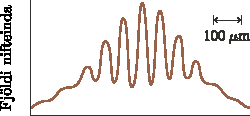
\includegraphics[width = 1.5in]{figures/fjoldi-nift.pdf}
\end{wrapfigure}

\item[\textbf{(38.49)}] Nifteindum með mjög lítinn hraða var beint í gegnum tveggja raufa raufagler með raufabil \SI{0.10}{mm} og samliðunarmynstrið var skoðað á skjá \SI{3.5}{m} fyrir aftan. Samliðunarmynstrið sem kom fram á skjánum má sjá á myndinni hér til hægri. Hver var hraði nifteindanna?

\end{minipage}

\item[\textbf{(38.48)}] Róteindum með hraða $\SI{0.99}{}c$ er beint í gegnum eina \SI{4}{nm} breiða rauf og bognunarmynstrið er skoðað á skjá \SI{50}{mm} fyrir aftan raufina. Hver verður breiddin á hámarkinu í miðjunni?

\begin{comment}
\item[\textbf{(38.56)}] Árið 1911 framkvæmdu Geiger og Mardsen hina frægu gullþynnutilraun fyrir doktorsleiðbeinanda sinn, Ernest Rutherford. Í tilrauninni beindu þeir $\alpha$-ögnum með hreyfiorku \SI{7.5}{MeV} í áttina að gullþynnu og komust að því að í sumum tilvikum þá endurköstuðust $\alpha$-agnirnar til baka. Þessi tilraun sýndi fram á tilvist kjarnans og róteindarinnar. Í greiningu sinni tók Rutherford ekki tillit til afstæðiskenningarinnar né skammtafræði. Hvers vegna var það í lagi?
\begin{enumerate*}[label = \textbf{(\alph*)}]
    \item Hver var de Broglie bylgjulengd $\alpha$-agnanna í gullþynnutilrauninni?
    \item Hver er geisli gullkjarnans?
    \item 
\end{enumerate*}
\end{comment}

\end{enumerate}

\begin{tcolorbox}
\begin{enumerate*}[label = ]
  \item \textbf{(38.16)} $\SI{1.1e-34}{m}$, $\SI{0.33}{nm}$, $\SI{3.6e6}{m/s}$.
  \item \textbf{(38.47)} $\SI{5.4}{\mu m}$.
  \item \textbf{(38.49)} $\SI{209}{m/s}$
  \item \textbf{(38.48)} $\SI{4.7}{nm}$.
\end{enumerate*}
\end{tcolorbox}

\newpage

\subsection*{Dæmatími 45: Inngangur að skammtafræði: Bohr-líkanið}

\begin{tcolorbox}
Árið 1913 setti Niels Bohr fram tilgátu um að hverfiþungi rafeinda væri skammtaður, $L = n\hbar$. Það hefur í för með sér að brautargeislar rafeinda verða skammtaðir og fyrir vetnisatómið er:
\begin{align*}
    r_n = a_{\!_B}n^2, \hspace{0.5cm} v_n = \frac{v_1}{n}, \hspace{0.5cm} E_n = \frac{E_1}{n^2}
\end{align*}
Þar sem að $a_{\!_B} = a_1 = \SI{0.529}{\AA}$ er Bohr-geislinn, $v_1 = \alpha c = \SI{2.19e6}{m/s}$ ($\alpha = \frac{1}{137}$ er fíngerðarfastinn) og $E_1 = \SI{-13.6}{eV}$ er grunnástand vetnisatómsins. Atómið gleypir eða geislar frá sér ljósi við það að rafeindir fara á milli brautargeisla. Við það losnar/gleypist ljóseind með orku $E_\gamma = \Delta E_{\text{atóm}}$. Fyrir stökk á milli orkuástanda $n$ og $m$ verður bylgjulengd ljóseindarinnar að vera (gildir bara fyrir vetni):
\begin{align*}
    \lambda_{nm} = \frac{\lambda_0}{\left( \frac{1}{n^2} - \frac{1}{m^2}\right)}, \hspace{1cm} \text{þar sem að} \hspace{0.5cm} \lambda_0 = \SI{91.18}{nm}.
\end{align*}
\end{tcolorbox}

\begin{enumerate}[label = \textbf{(\alph*)}]



\item[\textbf{(38.31)}] Skoðum vetnisatómið, $\ce{^{1}_{1}H}$.
\begin{enumerate}[label = \textbf{(\alph*)}]
    \item Hver er brautargeisli rafeindar sem hefur hraða \SI{7.3e5}{m/s}? Hver er skammtatala hennar?
    \item Hver er brautargeisli rafeindar sem hefur heildarorku \SI{-0.378}{eV}? Hver er skammtatala hennar?
    \item Hver þyrfti skammtatala rafeindar að vera til þess að geisli brautarinnar væri \SI{4}{\mu m}?
\end{enumerate}

\begin{minipage}{\linewidth}
\begin{wrapfigure}{r}{2.2in}
\vspace{-0.5cm}
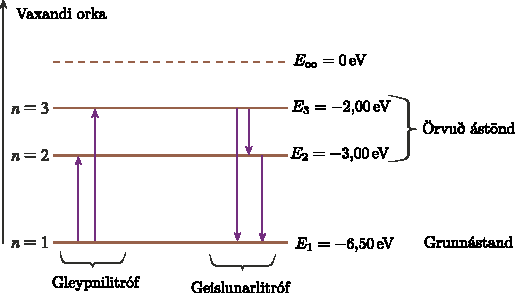
\includegraphics[width = 2.7in]{figures/gleipni.pdf}
\end{wrapfigure}

\item[\textbf{(38.56)}] Á myndinni hér til hægri má sjá orkumynd sem sýnir þrjú lægstu orkuástöndin fyrir óþekkt frumefni sem er ekki vetni.
\begin{enumerate}[label = \textbf{(\alph*)}]
    \item Hver er minnsta orkan sem þarf til þess að örva atómið?
    \item Hvaða bylgjulengdir koma fyrir í gleypnilitrófi atómsins?
    \item Hvaða bylgjulengdir koma fyrir í geislunarlitrófi atómsins?
\end{enumerate}

\end{minipage}

\vspace{1cm}

\item[\textbf{(38.59)}] Sýnilega litrófið sem að mannsaugað getur greint samanstendur af ljósi með bylgjulengd $\lambda \in [400; 750] \, \si{nm}$. Geislunarlitróf vetnis samanstendur af öllum þeim bylgjulengdum sem vetni getur geislað frá sér við það fara niður um orkuástand. Ákvarðið bylgjulengdirnar í sýnilega hluta geislunarlitrófs vetnis.


\item[\textbf{(38.62)}] Helstu orsökin fyrir því að ljós ferðast hægar í mismunandi efnum er sú að við það að ljóseindir lenda í árekstri við atóm í grunnástandi sínu þá örvast atómið upp í hærra orkustig. Skoðum vetnisatóm sem gleypir ljóseind og örvast upp í $n=2$ ástand. Atóm vilja hinsvegar að eðlisfari vera í orkulægsta ástandi sínu, grunnástandinu, $n=1$, og tíminn sem líður þar til að rafeindin geislar aftur frá sér ljóseind er að meðaltali \SI{1.6}{ns} (þetta er líkindaferli). Hversu marga snúninga snýst örvaða rafeindin umhverfis kjarnann á þessum tíma?

\end{enumerate}

\begin{tcolorbox}
\begin{enumerate*}[label = ]
  \item \textbf{(38.31)} $r_a = \SI{4.8}{\AA}$, $n_a = 3$, $r_b = \SI{1.9}{nm}$, $n_b = 6$, $n_c = 275$.
  \item \textbf{(38.56)} $\SI{3.5}{eV}$, $\lambda_b \in \left\{ \SI{355}{nm}, \SI{276}{nm}  \right\}$, $\lambda_c \in \left\{ \SI{355}{nm}, \SI{276}{nm}, \SI{1241}{nm}  \right\}$.
  \item \textbf{(38.59)} $\lambda_H \in \left\{ \SI{656.5}{nm}, \SI{486.3}{nm}, \SI{434.2}{nm}, \SI{410,3}{nm} \right\}$. \\
  \item \textbf{(38.62)} $\SI{1.05e7}{snúningar}$.
\end{enumerate*}
\end{tcolorbox}

\newpage

\subsection*{Dæmatími 46: Inngangur að skammtafræði: Óendanlegur mættisbrunnur}

\begin{tcolorbox}
Skoðum ögn með massa $m$ sem hefur hraða $v$ inni í kassa með lengd $\ell$. Vegna bylgjueiginleika efnisagna þá verður de Broglie bylgjulengdin $\lambda = \frac{h}{p}$. En þessu má líka við staðbylgju með lokuð jaðarskilirði svo bylgjulengdirnar verða skammtaðar, $\lambda_n = \frac{2 \ell}{n}$, en það gefur að heildarorkan verður:
\begin{align*}
    E_n = \frac{1}{2}mv_n^2  = \frac{h^2 n^2}{8m\ell^2}.
\end{align*}
Bylgjuföllin eru síðan gefin með:
\vspace{-0.6cm}
\begin{align*}
    \psi_n(x) = A\sin(k_n x),
\end{align*}
þar sem að 
\vspace{-0.4cm}
\begin{align*}
     k_n = \frac{2\pi}{\lambda_n} = \frac{n\pi}{\ell}, \hspace{1cm} \text{og stöðlunarfastinn er} \hspace{0.5cm} A = \sqrt{\frac{2}{\ell}}.
\end{align*}
Líkurnar á því að finna ögnina á bilinu $[a,b] \subseteq [0,\ell]$ eru gefnar með:
\begin{align*}
    \mathds{P}_{[a,b]} = \int_{a}^{b} \abs{\psi(x)}^2 dx
\end{align*}
\end{tcolorbox}

\begin{enumerate}[label = \textbf{(\alph*)}]

\item[\textbf{(38.51)}] Mýeindin er öreind sem svipar til rafeindarinnar. Mýeindin hefur sömu hleðslu og rafeindin en er $207$ sinnum massameiri. Hugsum okkur að við náum að fanga mýeind í flugnagildru af lengd \SI{70}{pm}. Eftir að við föngum mýeindina er hún í skammtaástandi $n = 3$ en fellur skömmu síðar niður í grunnástandið og geislar við það frá sér ljóseind. Hver er bylgjulengd ljóseindarinnar?

\item[\textbf{(38.22)}] Einfalt líkan af atómkjarnanum segir að kjarneindirnar séu bundnar í kassa með sömu lengd og þvermál atómkjarnans. Í einhverjum skilningi er hægt að segja að stöðugasta frumefnið sé járn, $\ce{_{26}^{56}Fe}$.
\begin{enumerate}[label = \textbf{(\alph*)}]
    \item Hver er orka kjarneindanna í grunnástandinu inni í járnkjarnanum?
    \item Frumeindamassi járns er $m_{\text{Fe}} = 55,934940u$. Bindiorka kjarnans er skilgreind sem stærðin:
    \begin{align*}
        \Delta E_B = -\left( m_{\text{Fe}} - Zm_p - Z m_e - (A-Z)m_n\right)c^2
    \end{align*}
    Með $m_p = 1,00728u$, $m_e = 0,00055u$, $m_n = 1,00866u$ og $u = \SI{1.6605e-27}{kg} = \SI{931.49}{\frac{MeV}{c^2}}$. Hver er bindiorka járnkjarnans? Hver er bindiorkan per kjarneind ($\Delta E_B / A$) í járnkjarnanum? Er þetta meira eða minna heldur en svarið í \textbf{(a)}-lið?
\end{enumerate}


\item[\textbf{(40.27)}] Vatnsdropi með geisla \SI{1.0}{\mu m} rúllar með hraða \SI{1.0}{\mu m/s} inni í núningslausum kassa af lengd \SI{20}{\mu m}. \begin{enumerate}[label = \textbf{(\alph*)}]
    \item Hver er skammtatala vatnsdropans?
    \item Ef skammtatala kerfis er mjög há þá er yfirleitt í lagi að lýsa kerfinu með klassískum aðferðum. Er það í lagi hér?
    \item Hverjar eru líkurnar á því að finna ögnina í \SI{2}{\mu m} fjarlægð frá öðrum hvorum endanum?
\end{enumerate}

\item[\textbf{(40.33)}] Skoðum ögn með massa $m$ í óendanlegum mættisbrunni af lengd $\ell$. 
\begin{enumerate}[label = \textbf{(\alph*)}]
    \item Hverjar eru líkurnar á því að finna ögn í grunnástandinu inni á bilinu $[0,\frac{\ell}{4}]$?
    \item Hverjar eru líkurnar á því að finna ögn í $n = 2$ skammtaástandinu inni á bilinu $[0,\frac{\ell}{4}]$?
    \item Hverjar eru líkurnar á því að finna ögn í grunnástandinu inni á bilinu $[\frac{\ell}{4}, \frac{\ell}{4} + b]$ þar sem að $b = \frac{\ell}{100}$?
\end{enumerate}

\begin{tcolorbox}
\begin{enumerate*}[label = ]
    \item \textbf{(38.51)} $\SI{418}{nm}$.
  \item \textbf{(38.22)} $\SI{2.4}{MeV}$, $\SI{492.2}{MeV}$, $\SI{8.8}{MeV}$.
  \item \textbf{(40.27)} $n = \SI{2.53e8}{}$, Já, \num{0.20}.
  \item \textbf{(40.33)} $\SI{0.091}{}$, $0,33$, $0,01$.
\end{enumerate*}
\end{tcolorbox}



\end{enumerate}

\newpage